\documentclass{scrartcl}
\usepackage[utf8]{inputenc}
\usepackage[english]{babel}
\usepackage{amsthm, amsmath, amssymb}
\usepackage{mathtools}
\usepackage{graphicx}
\usepackage{hyperref}

\newtheorem{task}{Task}
\newtheorem{claim}{Claim}

\begin{document}
	\title{Practical Lab - Computational Finance \\ Sheet 1}
	\author{Min Liu, Christian Fiedler and Tim Griesbach}
	\date{November 4th, 2019}
	\maketitle
	
	\section*{Simulate the normal distribution}
	\begin{task}
		What does the given code do? What is the difference between the two ways to generate random
		numbers? What happens if you remove the expression (double) in the line marked with // *? Look
		at the GSL reference and see whether there is a direct function for simulating normally distributed
		random variables.
	\end{task}
	% TODO: Difference: mt19937 und rand()/RAND_MAX
	The random number generator from GSL is a variant of the twisted generalized feedback shift-register algorithm (cited from reference). This random number generator pass also different statistical tests. $\texttt{rand()}$ is a simpler functions. That means we could expect that the gsl random number generator causes less biased results than the method via \texttt{rand()}. 
	The function \texttt{int rand(void)}
	returns a pseudo-random number in the range of 0 to \texttt{RAND\_MAX}.
	\texttt{RAND\_MAX} is a constant whose default value may vary 
	between implementations but it is granted to be at least 32767.\\
	Thus we can see  \texttt{(double)rand()/RAND\_MAX} as a random variable, which is unifomly distributed in [0,1]. Without "\texttt{(double)}" this number is just 0. This the case because the return type of \texttt{rand()} is \texttt{int}. So, this expression evaluates to zero because without the type casting the result has to be a \texttt{int}.\\
	The rest codes set a uniform distributed random variable and free the memory by using \texttt{gsl\_rng\_free}. In the gsl reference we can find followings for the normal distribution: 

	\begin{itemize}
		\item \texttt{double gsl\_ran\_gaussian(const gsl\_rng * r, double sigma) } This function returns a 
		Gaussian random variate, with mean zero and standard deviation sigma.
		\item \texttt{double gsl\_ran\_gaussian\_pdf(double x, double sigma) } This function computes the probability density $p(x)$ at $x$ for a Gaussian distribution with standard deviation sigma, 
		using the formula given above.
		\item \texttt{double gsl\_ran\_ugaussian(const gsl\_rng * r),\\
			double gsl\_ran\_ugaussian\_pdf(double x) and \\
			double gsl\_ran\_ugaussian\_ratio\_method(const gsl\_rng * r)}. These functions compute results for the unit Gaussian distribution. They are equivalent to the functions above with a standard deviation of one, sigma = 1.
	\end{itemize}
	
	\begin{task}
		Implement the rejection sampling algorithm in C/C++ and output 1 000 000 values into
		a file.
	\end{task}
	We draw uniformly distributed random variables in a intervall $[a,b]$ using the function \texttt{gsl\_rng\_uniform} and a bijection between $[0,1]$ and $[a,b]$. \\
	The rejection sampling is just the implementation of the given steps with the intervall $[-3,3]$ in step 1 since $\int_{-3}^{3}\frac{1}{\sqrt{2\pi}}\exp\left(-\frac{x^2}{2}\right) \approx 0.9973$. A too large intervall could increase the runtime because we could have more samples $x'$ with big $|x'|$. That means $p(x')$ will be small an we need in the mean more loops pass until the rejection sampling returns a value. 

	\begin{task}
		Inspect your data using MATLAB. What does the MATLAB script do? Do you get a
		sensible result? What did probably go wrong in Fig. 1?
	\end{task}
	The Matlab script reads the textfile \texttt{values.txt} in the current folder that should contain samples of a gaussian random variable. \\
	These samples are assigned to the variable \texttt{data} and then by the \texttt{[vals, bins] = hist(data, 100)} the samples are split into hundred bins. \texttt{vals} and \texttt{bins} are vectors. \texttt{vals} contains the frequency counts and \texttt{bins} contains the locations of the bins (centers of the corresponding intervall).  \\
	Then the standard gaussian density function is plotted and the frequency counts are also plotted. However, the frequency counts in \texttt{vals} are normalized by \texttt{trapz(bins, vals)} which approximates the integral of \texttt{vals} with respect to \texttt{bins}.
	The rest of the code just creates a legend and lables the axis.\\
		\begin{figure}[h]
			\centering
			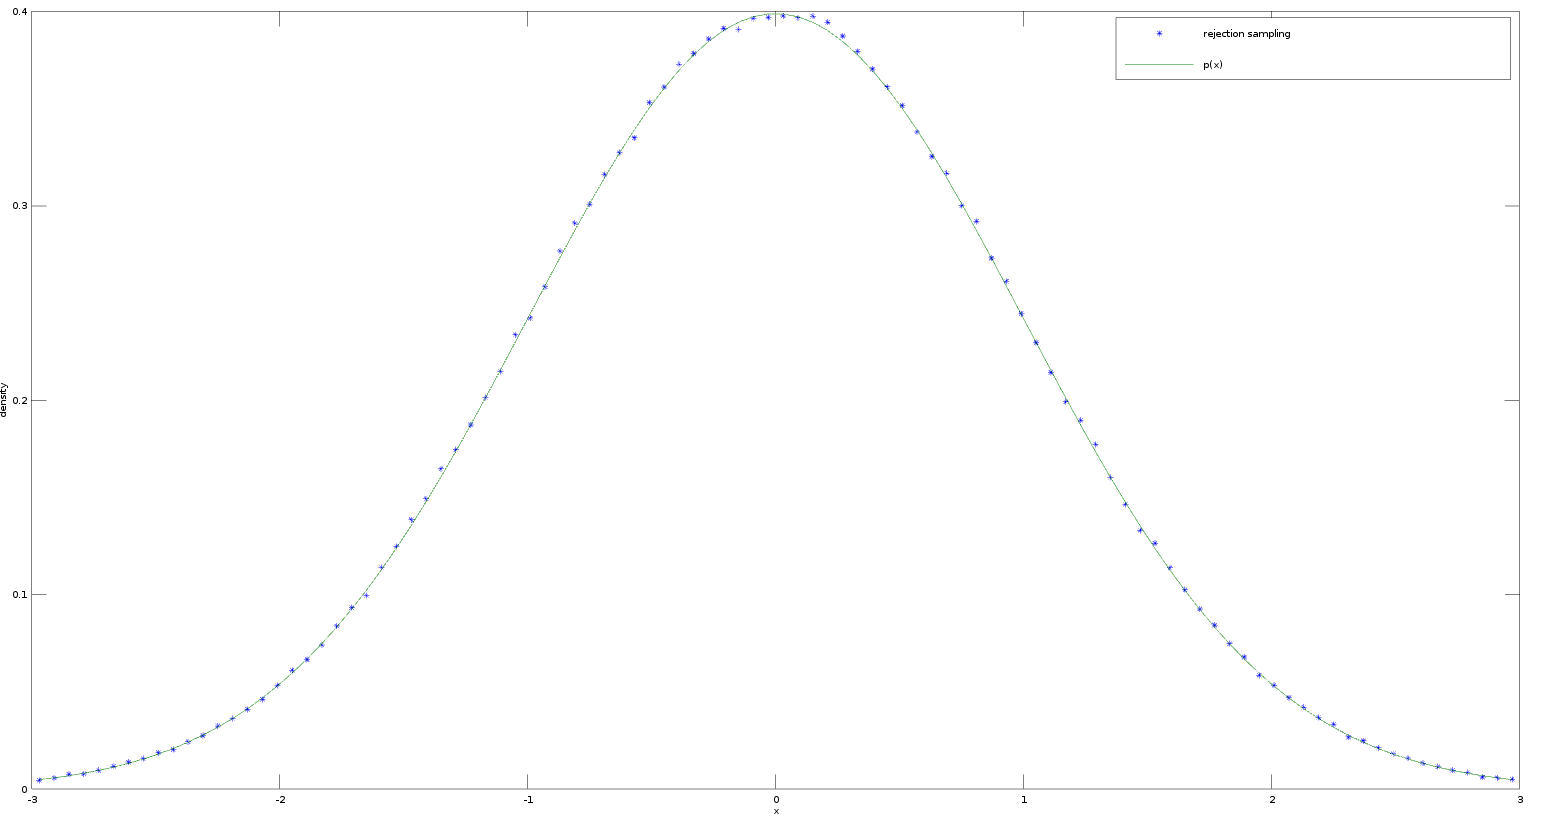
\includegraphics[width=0.8\textwidth]{plot_rejection_sampling}
			\caption{Output of the given Matlab script from task 3 if we use 1 000 000 samples in our rejection sampling implementation.}
			\label{fig_rejection_samp}
			\end{figure}
	Figure \ref{fig_rejection_samp} shows the output of the given Matlab script. We can observe that the samples generated with our rejection sampling implementation fits good to the gaussian density. \\
	In figure 1 from the sheet probably the intervall was chosen too small. This hypothesis is supported by the following plot in figure \ref{fig_rejection_samp_wrong} with our implementation of the rejection sampling and the intervall $[-2,2]$.
	\begin{figure}[h]
		\centering
		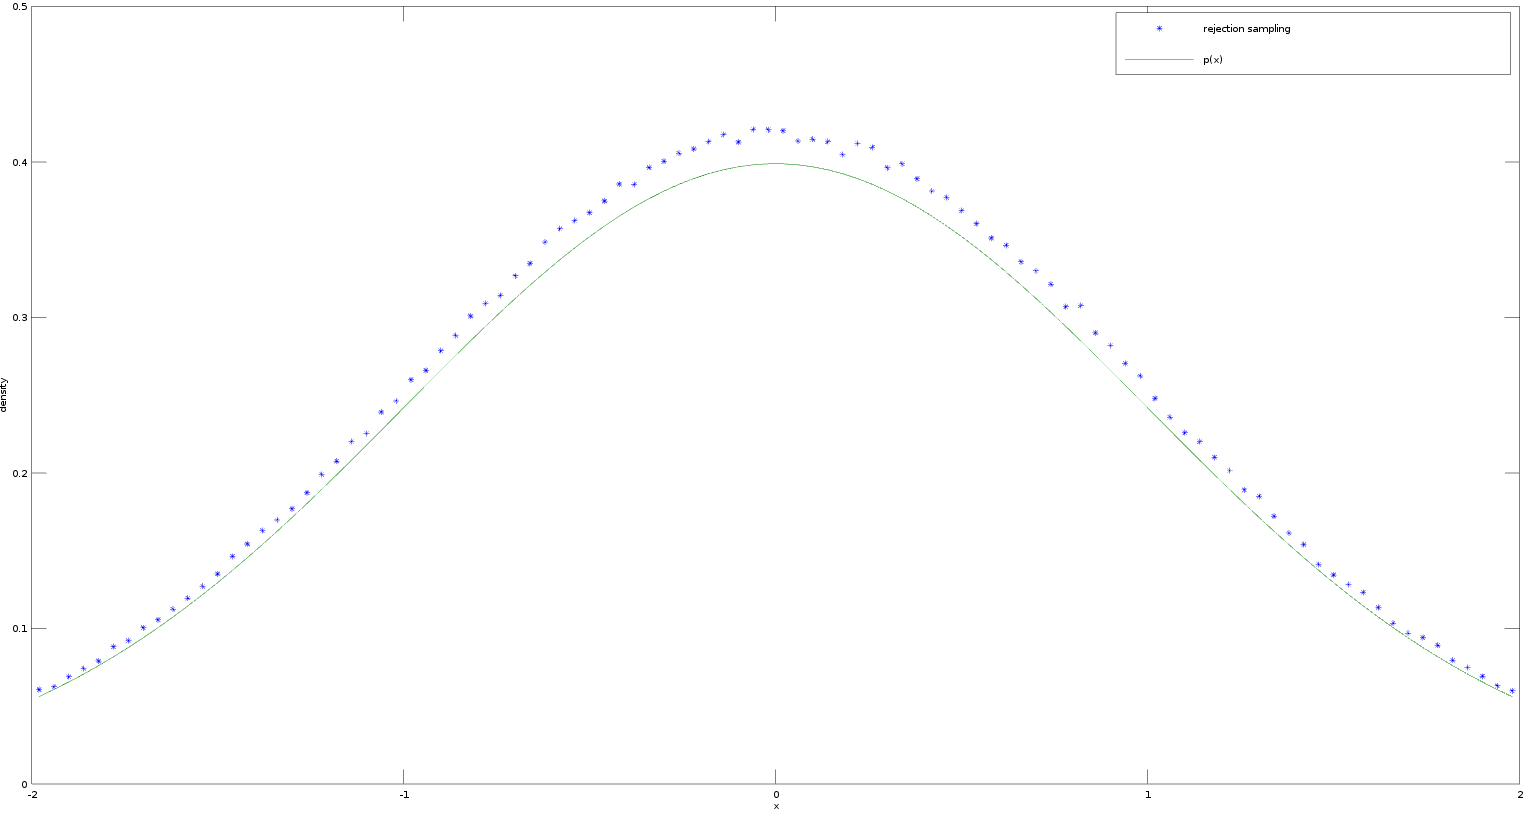
\includegraphics[width=0.8\textwidth]{rejection_sampling_too_small_intervall}
		\caption{Output of the given Matlab script from task 3 if we use 1 000 000 samples in our rejection sampling implementation and the intervall $[-2,2]$.}
		\label{fig_rejection_samp_wrong}
	\end{figure} 
	% Fig. 1: Perhaps the maximum was choosen to high or the seeds have systematic effect that is visible in this plot.
	
	\begin{task}
		How do you get a normally distributed random variable when you only have a uniform
		one? Not entirely by coincidence, the c.d.f. and inverse c.d.f. of the standard normal distribution
		are computed by the two algorithms given below. Implement both algorithms and write a program
		that draws standard normal distributed values.
	\end{task}

	\begin{claim}
		For a random variable $X$, its cumulative distribution function $F_x : \mathbb{R} \to [0,1]$ and the generalized inverse cumulative distribution function $F_X^{-1} : [0,1] \to \mathbb{R}\cup\{-\infty, +\infty\}$ with $F_X^{-1}(y)=\inf_{x\in\mathbb{R}}\{F_X(x)\geq y\}$ holds:
		If $U\sim\textrm{Unif}([0,1])$, then
		\begin{equation}
			F_X^{-1}(U)\sim X.
		\end{equation}
	\end{claim}
	\begin{proof}
		We define $\tilde{X}\coloneqq F_X^{-1}(U)$. For $x\in\mathbb{R}$ we get
		\begin{align}
			F_{\tilde{X}}(x) &= P\left[F_X^{-1}(U) \leq x\right] = P\left[\inf_{x'\in\mathbb{R}}\{F_X(x')\geq U\} \leq x\right] \\
			&= P\left[U \leq F_X(x)\right] = F_X(x). 
		\end{align}
	\end{proof}
	The implementation of the approximation algorithms for the c.d.f. and the inverse c.d.f. were already given on the sheet. \\
	We can just apply the inverse c.d.f to draw standard normal distributed random variables to a realization of a standard uniform distributed random variable. See figure \ref{fig_moro_samp} for a result.
	\begin{figure}[h]
		\centering
		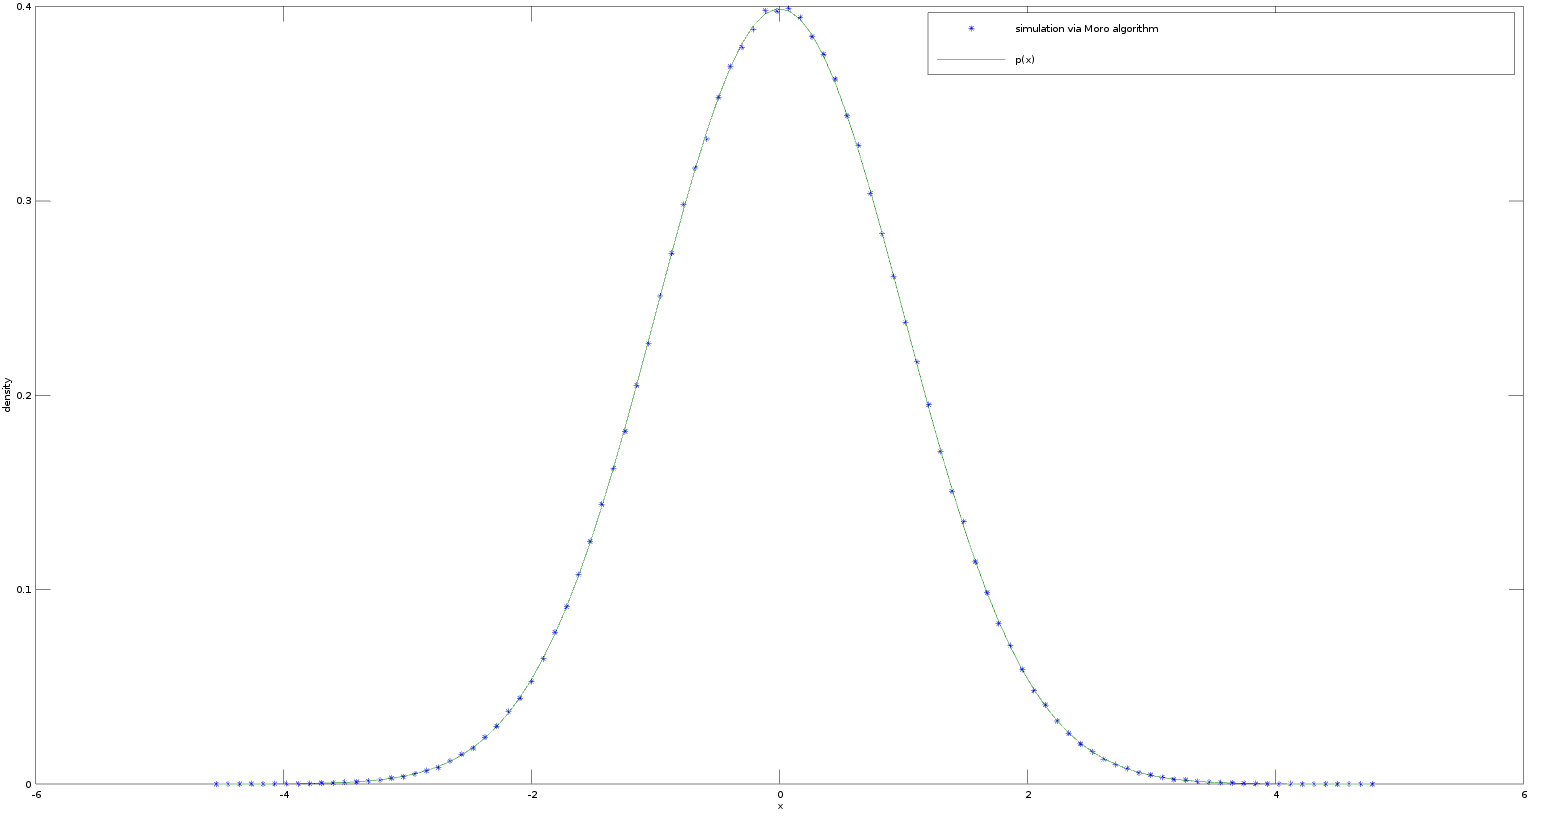
\includegraphics[width=0.8\textwidth]{samples_moro}
		\caption{Output of the given Matlab script from task 3 if we use 1 000 000 samples in our simulation of a standard normal random variable using the idea explainded in our answer to task 4.}
		\label{fig_moro_samp}
	\end{figure}
	
	\begin{task}
		Explain the general idea behind Moro’s algorithm!
	\end{task}
	According to the sheet Moro's algorithm is an approximation to the c.d.f. of the standard normal distribution. \\
	The general idea behind the given algorithm is to approximate the c.d.f. of the standard normal piecewise with a rational functions that are evaluated by Horner's method (linear number of multiplications and summations in polynomials degrees). \\
	For negative evaluation points $x$ the algorithm uses that for $X\sim N(0,1)$ 
	\begin{equation}
		F_X(x) = 1 - F_X(-x)
	\end{equation}
	holds.
	Now for different remaining ranges are different rational functions used to approximate the c.d.f.. 

	\begin{task}
		Implement the Box-Muller method and plot 1 000 samples in a 2d-plot.
	\end{task}
	For the implementation we use the given expressions for $Z_1, Z_2$ from the sheet and generate standard uniform samples with the GSL libary. \\
	In figure \ref{fig_box_muller_1000} we can oberserve that the samples are concentrated in a circle with radius two around $(0,0)$. That is exactly what we expect if we look at the density function of $(Z_1, Z_2)$. This obervation become clearer if we consider the 10 000 samples with the same seed as in figure \ref{fig_box_muller_10000}.
	\begin{figure}[h]
		\centering
		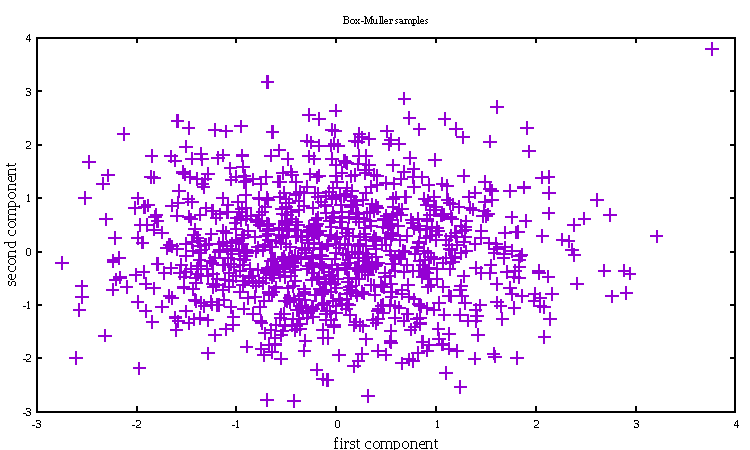
\includegraphics[width=0.8\textwidth]{Box-Muller}
		\caption{2d plot of the 1 000 samples generated with the box muller method.}
		\label{fig_box_muller_1000}
	\end{figure}
	\begin{figure}[h]
		\centering
		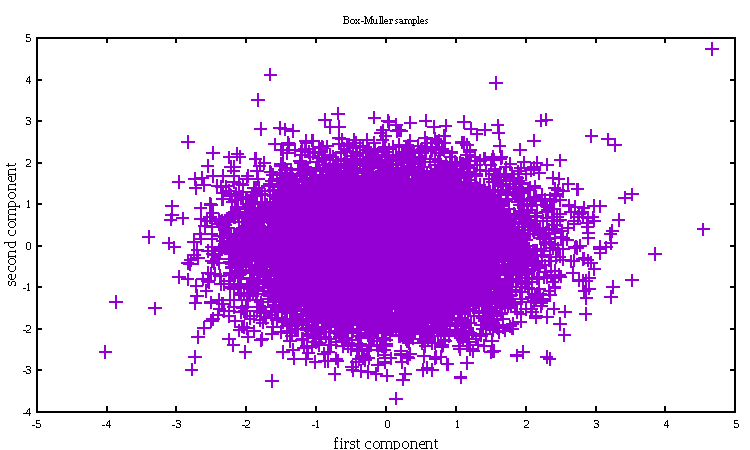
\includegraphics[width=0.8\textwidth]{Box-Muller_10000_samples}
		\caption{2d plot of the 10 000 samples generated with the box muller method. The seed is the same as in figure \ref{fig_box_muller_1000}.}
		\label{fig_box_muller_10000}
	\end{figure}
	
	\begin{task}
		Do some research and be prepared to explain why $z_1$ and $z_2$ are standard normally distributed.
	\end{task}
	\begin{claim}
		If $U_1, U_2 \sim \textrm{Unif([0,1)}$ are independent, then $Z_1, Z_2 \sim N(0,1)$ i.i.d. where
		\begin{align}
			Z_1 &\coloneqq \sqrt{-2\log U_1}\cos(2\pi U_2), \\
			Z_2 &\coloneqq \sqrt{-2\log U_1}\sin(2\pi U_2).
		\end{align}
	\end{claim}
	\begin{proof}
		Let $U_1$ and $U_2$ be random variables with $U_1, U_2 \sim \textrm{Unif}([0,1))$. We define
		\begin{equation}
		R \coloneqq \sqrt{-2\log U_1} \quad \text{and} \quad \Phi \coloneqq 2\pi U_2.
		\end{equation}
		Then we apply change of variable to the transformation
		\begin{equation}
		\psi : \mathbb{R}_{>0} \times [0,2\pi) \to \mathbb{R} \times \mathbb{R}, \quad (r,\phi) \mapsto (r\cos\phi, r\sin\phi)
		\end{equation}
		and we obtain that for the density function of
		\begin{equation}
		(Z_1, Z_2) \coloneqq (R\cos\Phi, R\sin\Phi)
		\end{equation}
		holds for $x = r\cos\phi$ and $y = r\sin\phi$
		\begin{equation}
		f_{Z_1,Z_2}(x,y) = \underbrace{f_{R,\Phi}(r,\phi)}_{\overset{(\star)}{=}\frac{1}{2\pi} r\exp\left(-\frac{r^2}{2}\right)} \underbrace{\frac{1}{\det D\psi}}_{=\frac{1}{r}} = \frac{1}{2\pi}\exp\left(-\frac{x^2+y^2}{2}\right)
		\label{eq_joint_density}
		\end{equation}
		The equality $(\star)$ is satisfied because for $r\in\mathbb{R}_{>0}$
		\begin{equation}
			P[R\leq r] = P[\sqrt{-2\log U_1} \leq r] = P\left[U_1\geq \exp\left(-\frac{r^2}{2}\right)\right] = 1 - \exp\left(-\frac{r^2}{2}\right).
		\end{equation}
		That is why we get as density function of the random variable $R$
		\begin{equation}
			f_R(r) = r\exp\left(-\frac{r^2}{2}\right).
		\end{equation}
		By assumptions $U_1$ and $U_2$ are independent that implies that $R$ and $\Phi$ are independent. That means with $\Phi\sim\textrm{Unif}([0,2\pi))$ we obtain for $r\in\mathbb{R}_{>0}$ and $\phi\in[0,2\pi)$
		\begin{equation}
			f_{R,\Phi}(r,\phi) = r\exp\left(-\frac{r^2}{2}\right)\frac{1}{2\pi}
		\end{equation}
		as density function of $(R,\Phi)$. \\
		By factorization of the density function in equation \ref{eq_joint_density} we get that $Z_1$ and $Z_2$ are independent and $Z_1, Z_2 \sim N(0,1)$.
	\end{proof}
	
	\section*{Parameter estimation}
	\begin{task}
		Compute \ref{eq_sigma_est} naively and show experimentally that it yields the same result as the given
		algorithm. What is the advantage of this algorithm?
		\begin{align}
			\hat{\mu} &= \frac{1}{N}\sum_{i=1}^{N}x_i \\
			\hat{\sigma}^2 &= \frac{1}{N-1}\sum_{i=1}^{N}(x_i-\hat{\mu})
			\label{eq_sigma_est}
		\end{align}
	\end{task}
	% TODO: Naiven Vergleich programmieren und den Vorteil des gegeben Ansatzes erklären.
	They can get the same results, since $\alpha$ in the i-th for-loop is just the mean value of the first i components and sigma is just the variation of first i components.\par 
	The second is better, since it decompose more complex computation intp several easy computation such that rounding errors are less problematic.
	
	%\section*{Task 9: Convergence plot of the estimation error}
	\begin{task}
		Choose an arbitrary $\mu$ and three different values for $\sigma$. Simulate N (up to N max =
		10 000 000) samples by (6) and calculate $\hat{\sigma}$ for each of the three values of $\sigma$. Now generate a loglog-
		convergence plot (e.g. with GNUPLOT, MATLAB, matplotlib, pgfplots, . . .) of the estimation error
		$|\sigma-\hat{\sigma}|$ (for each $\sigma$) with respect to the number of samples N used for parameter estimation in the
		fashion of Fig. 2. How do you interpret the result?
	\end{task}
	In our convergence plot we see that for bigger $\sigma$ the estimation error is bigger (with a few exceptions). This coincides roughly with the observations from figure 1 and 2 from the sheet.
	Furthermore, we can observe a linear decreasing trend in the plot and since figure \ref{fig_conv_plot_est_sigma} has two log-scaled axis the estimation error decreases exponetially in the number of samples $N$ (see also the plotted function $l(N)=N^{-0.6}$).
	\begin{figure}[h!]
		\centering
		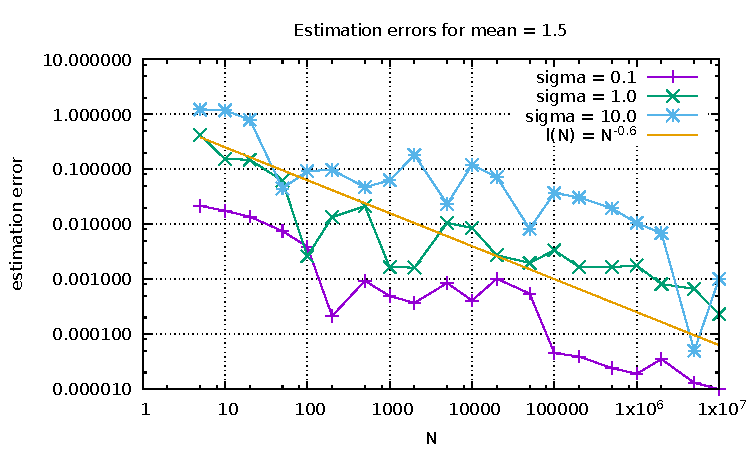
\includegraphics[width=\textwidth]{convergence_plot_sigma_estimation}
		\caption{A plot of the estimation error with different $\sigma$ and a fixed $\mu$. The axis are $\log$-scaled. Moreover, $N$ is the number of samples.}
		\label{fig_conv_plot_est_sigma}
	\end{figure}
	
	% Beachte Verhältnis von Erwartungswert und Varianz sowie verhältnismäßig kurze Zeitspanne (2 Jahre).
	\section*{Simulating and calibrating geometric Brownian motions}
	\begin{task}
		We set S(0) = 10, $\mu$ = 0.1, $\sigma$ = 0.2, T = 2. Simulate 3 paths of a Wiener process with (2)
		and the corresponding asset prices (3) for $\Delta t$ = 0.5 and 3 paths for $\delta t$ = 0.01.Do the paths in principial look the same, independent of the time discretization? Is the
		mean change of the price S(t) approximately +0.1/year?
	\end{task}
	The paths do not look in the same (compare figures \ref{fig_wiener} and \ref{fig_gbm}), independent of the time steps. This is the case because we only get a very rough approximation (piecewise) of one sample and the number evaluations of the single standard normal distributed random variables differs. That is we do not get the same value for the time $1$ even with both time steps we get a value for this time. \\
	The mean change of the price $S(t)$ holds roughly in figure \ref{fig_gbm}. We can see this because of the plottes mean ($10\exp(0.1  x)$). However, this hols only roughly. This can be explained by the fact that for two years and a mean of $0.1$ is a standard deviation of $0.2$ quite high. Furthermore three paths are not enough to make a profound statment. 
	
	\begin{figure}[h!]
		\centering
		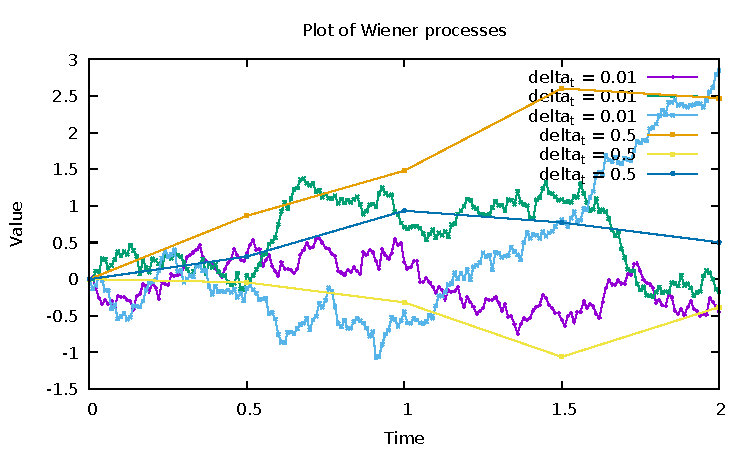
\includegraphics[width=\textwidth]{wiener}
		\caption{A plot three paths of the Wiener process with $\mu = 0.1$ and $\sigma = 0.2$ for different time steps (0.5 and 0.01).}
		\label{fig_wiener}
	\end{figure}
	\begin{figure}[h!]
		\centering
		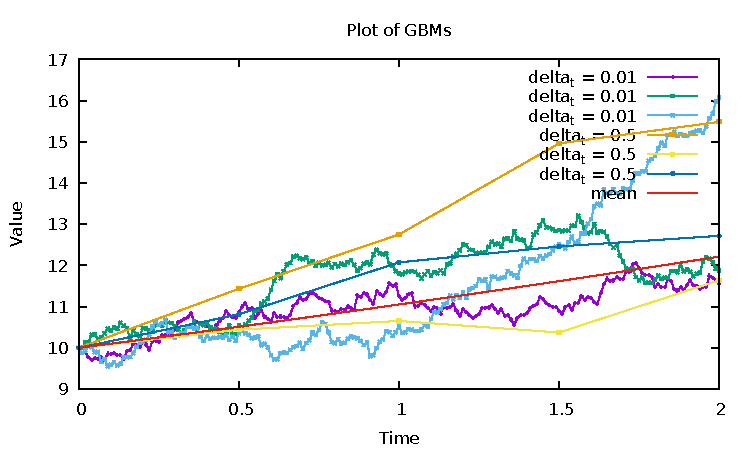
\includegraphics[width=\textwidth]{gbm}
		\caption{A plot three paths of the geometric Brownian motion with $S(0) = 10$, $\mu = 0.1$ and $\sigma = 0.2$ for different time steps (0.5 and 0.01).}
		\label{fig_gbm}
	\end{figure}
	
	\begin{task}
		Similar to Task 10, simulate a geometric Brownian motion with parameters S(0) = 10, $\mu$ = 0.1, $\sigma$ =
		0.2, T = 1 and $\Delta t = 10^{-3}$ . Given the values of S(0), T and $\Delta t$, estimate the values of $\mu$ and $\sigma$
		from the 1000 time steps of your simulation. Explain your approach.
	\end{task}
	The idea behind our approach is that the $\log$-returns are normally distributed. In particular,
	\begin{equation}
		\log\left(\frac{S(t)}{S(0)}\right) = \left(\mu - \frac{1}{2}\sigma^2\right)t + \sigma W(t).
	\end{equation} 
	This means $\log\left(\frac{S(t)}{S(0)}\right) \sim N(\left(\mu - \frac{1}{2}\sigma^2\right)t, \sigma^2 t)$. Now we want to get rid of the dependence from $t$. That is why we consider
	\begin{equation}
		\log\left(\frac{S(t_i)}{S(t_{i-1})}\right) \sim N\left(\left(\mu - \frac{1}{2}\sigma^2\right)(t_i - t_{i-1}), \sigma^2 (t_i - t_{i-1})\right).
	\end{equation}
	Now estimate $\mu$ and $\sigma$ as in task 8 what gives estimates for $\sigma$ and $\mu$ after rewrite the equality of the $\log$-return estimated and the above derived mean and standard deviation for time steps. \\
	This approach is also implemented in our code.
	
\end{document}